\chapter{Dynamic Constraints of a UAV}
\label{chp:Dynamic}

% Include thing where you compare distance measures and how it effects number of rotations
% Include thing where you add spanning tree weights to reduce number of rotations
% Address energy consumption

\tikzset{every picture/.style={line width=0.75pt}} %set default line width to 0.75pt        

\begin{figure}[h!]
	\centering 
	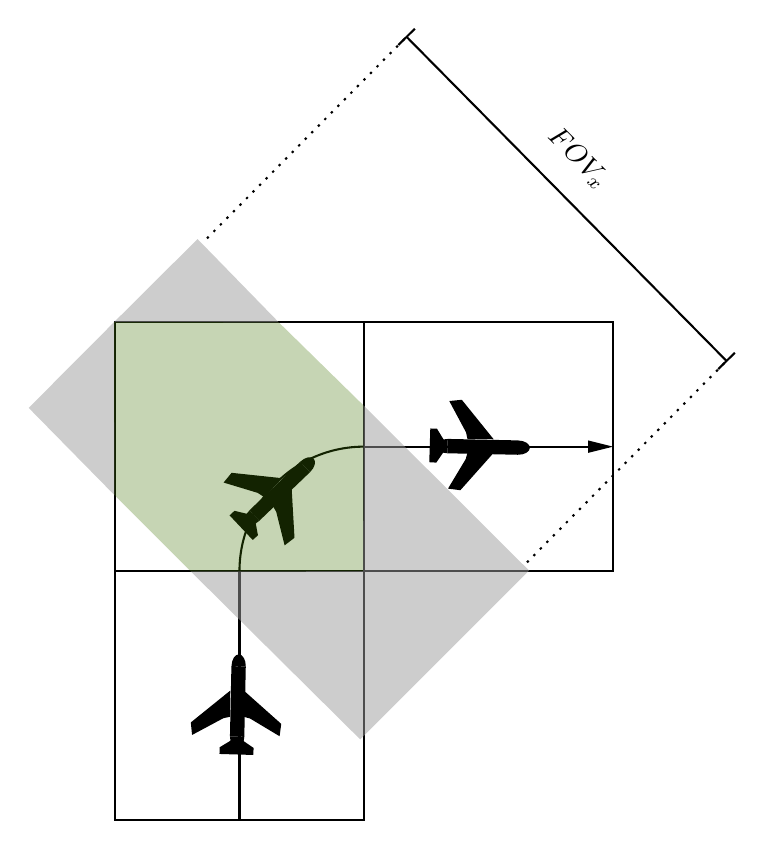
\begin{tikzpicture}[x=0.75pt,y=0.75pt,yscale=-1,xscale=1]
	%uncomment if require: \path (0,483); %set diagram left start at 0, and has height of 483
	
	%Shape: Square [id:dp7554025064162504] 
	\draw  [line width=0.75]  (184.88,300) -- (304.88,300) -- (304.88,420) -- (184.88,420) -- cycle ;
	%Shape: Square [id:dp029527299824832154] 
	\draw  [line width=0.75]  (184.88,180) -- (304.88,180) -- (304.88,300) -- (184.88,300) -- cycle ;
	%Shape: Square [id:dp05898723469860556] 
	\draw  [line width=0.75]  (304.88,180) -- (424.88,180) -- (424.88,300) -- (304.88,300) -- cycle ;
	%Straight Lines [id:da2896157813713012] 
	\draw [line width=0.75]    (244.88,300) -- (244.88,420) ;
	%Straight Lines [id:da6458424182642684] 
	\draw [line width=0.75]    (422.88,240) -- (304.88,240) ;
	\draw [shift={(424.88,240)}, rotate = 180] [fill={rgb, 255:red, 0; green, 0; blue, 0 }  ][line width=0.08]  [draw opacity=0] (12,-3) -- (0,0) -- (12,3) -- cycle    ;
	%Shape: Arc [id:dp6697923261787817] 
	\draw  [draw opacity=0][line width=0.75]  (244.88,300) .. controls (244.88,266.86) and (271.74,240) .. (304.88,240) -- (304.88,300) -- cycle ; \draw  [line width=0.75]  (244.88,300) .. controls (244.88,266.86) and (271.74,240) .. (304.88,240) ;
	%Shape: Chord [id:dp19722764417953975] 
	\draw  [draw opacity=0][fill={rgb, 255:red, 0; green, 0; blue, 0 }  ,fill opacity=1 ][line width=0.75]  (274.12,247.29) .. controls (276.41,245.09) and (279.34,244.42) .. (280.66,245.79) .. controls (281.97,247.17) and (281.18,250.07) .. (278.88,252.27) -- cycle ;
	%Shape: Rectangle [id:dp7564053950991294] 
	\draw  [draw opacity=0][fill={rgb, 255:red, 0; green, 0; blue, 0 }  ,fill opacity=1 ][line width=0.75]  (278.88,252.27) -- (254.42,275.73) -- (249.64,270.73) -- (274.1,247.27) -- cycle ;
	%Shape: Chord [id:dp8544272377140341] 
	\draw  [draw opacity=0][fill={rgb, 255:red, 0; green, 0; blue, 0 }  ,fill opacity=1 ][line width=0.75]  (254.42,275.73) .. controls (254.42,275.73) and (254.42,275.73) .. (254.42,275.73) .. controls (252.12,277.93) and (249.2,278.6) .. (247.88,277.22) .. controls (246.57,275.85) and (247.36,272.95) .. (249.66,270.75) -- cycle ;
	%Shape: Boxed Polygon [id:dp4243302902770245] 
	\draw  [draw opacity=0][fill={rgb, 255:red, 0; green, 0; blue, 0 }  ,fill opacity=1 ][line width=0.75]  (266.64,287.56) -- (262.59,271.38) -- (261.02,268.73) -- (270.02,260.03) -- (271.39,283.91) -- cycle ;
	%Shape: Boxed Polygon [id:dp6815588587808861] 
	\draw  [draw opacity=0][fill={rgb, 255:red, 0; green, 0; blue, 0 }  ,fill opacity=1 ][line width=0.75]  (237.24,257.3) -- (253.63,262.26) -- (256.31,264) -- (265.4,255.2) -- (241.08,252.61) -- cycle ;
	%Shape: Boxed Polygon [id:dp4894660411365015] 
	\draw  [draw opacity=0][fill={rgb, 255:red, 0; green, 0; blue, 0 }  ,fill opacity=1 ][line width=0.75]  (253.78,282.71) -- (251.27,284.96) -- (240.12,273.11) -- (242.5,270.91) -- (252.04,273.24) -- cycle ;
	
	%Shape: Boxed Line [id:dp4808926265834552] 
	\draw  [dash pattern={on 0.84pt off 2.51pt}]  (229.24,139.64) -- (325.41,42.57) ;
	%Straight Lines [id:da17659301005268957] 
	\draw [line width=0.75]    (325.41,42.57) -- (479.55,198.71) ;
	\draw [shift={(479.55,198.71)}, rotate = 225.37] [color={rgb, 255:red, 0; green, 0; blue, 0 }  ][line width=0.75]    (0,5.59) -- (0,-5.59)   ;
	\draw [shift={(325.41,42.57)}, rotate = 225.37] [color={rgb, 255:red, 0; green, 0; blue, 0 }  ][line width=0.75]    (0,5.59) -- (0,-5.59)   ;
	%Shape: Boxed Line [id:dp01374331482035851] 
	\draw  [dash pattern={on 0.84pt off 2.51pt}]  (383.38,295.78) -- (479.55,198.71) ;
	%Shape: Chord [id:dp9231747485755666] 
	\draw  [draw opacity=0][fill={rgb, 255:red, 0; green, 0; blue, 0 }  ,fill opacity=1 ][line width=0.75]  (241.03,345.76) .. controls (241.03,345.76) and (241.03,345.76) .. (241.03,345.76) .. controls (241.1,342.58) and (242.69,340.03) .. (244.6,340.08) .. controls (246.5,340.12) and (247.99,342.73) .. (247.92,345.91) -- cycle ;
	%Shape: Rectangle [id:dp34380596609036296] 
	\draw  [draw opacity=0][fill={rgb, 255:red, 0; green, 0; blue, 0 }  ,fill opacity=1 ][line width=0.75]  (247.92,345.91) -- (247.21,379.79) -- (240.29,379.64) -- (241,345.76) -- cycle ;
	%Shape: Chord [id:dp3433894979507466] 
	\draw  [draw opacity=0][fill={rgb, 255:red, 0; green, 0; blue, 0 }  ,fill opacity=1 ][line width=0.75]  (247.21,379.8) .. controls (247.21,379.8) and (247.21,379.8) .. (247.21,379.8) .. controls (247.21,379.8) and (247.21,379.8) .. (247.21,379.8) .. controls (247.14,382.98) and (245.55,385.52) .. (243.65,385.48) .. controls (241.74,385.44) and (240.26,382.82) .. (240.32,379.64) -- cycle ;
	%Shape: Boxed Polygon [id:dp08898175934962804] 
	\draw  [draw opacity=0][fill={rgb, 255:red, 0; green, 0; blue, 0 }  ,fill opacity=1 ][line width=0.75]  (264.22,379.52) -- (249.92,370.95) -- (246.93,370.18) -- (247.14,357.67) -- (265,373.58) -- cycle ;
	%Shape: Boxed Polygon [id:dp8735831522150785] 
	\draw  [draw opacity=0][fill={rgb, 255:red, 0; green, 0; blue, 0 }  ,fill opacity=1 ][line width=0.75]  (222.04,378.91) -- (237.13,370.83) -- (240.25,370.17) -- (240.46,357.52) -- (221.43,372.88) -- cycle ;
	%Shape: Boxed Polygon [id:dp35625726838667515] 
	\draw  [draw opacity=0][fill={rgb, 255:red, 0; green, 0; blue, 0 }  ,fill opacity=1 ][line width=0.75]  (251.7,385.19) -- (251.51,388.55) -- (235.25,388.06) -- (235.37,384.82) -- (243.77,379.72) -- cycle ;
	
	%Shape: Chord [id:dp34828845330166835] 
	\draw  [draw opacity=0][fill={rgb, 255:red, 0; green, 0; blue, 0 }  ,fill opacity=1 ][line width=0.75]  (379.12,237.02) .. controls (379.12,237.02) and (379.12,237.02) .. (379.12,237.02) .. controls (382.3,237.09) and (384.85,238.69) .. (384.8,240.59) .. controls (384.76,242.49) and (382.15,243.98) .. (378.97,243.91) -- cycle ;
	%Shape: Rectangle [id:dp8474408050833497] 
	\draw  [draw opacity=0][fill={rgb, 255:red, 0; green, 0; blue, 0 }  ,fill opacity=1 ][line width=0.75]  (378.97,243.91) -- (345.09,243.2) -- (345.24,236.28) -- (379.12,236.99) -- cycle ;
	%Shape: Chord [id:dp5085353869793547] 
	\draw  [draw opacity=0][fill={rgb, 255:red, 0; green, 0; blue, 0 }  ,fill opacity=1 ][line width=0.75]  (345.09,243.2) .. controls (345.09,243.2) and (345.09,243.2) .. (345.09,243.2) .. controls (341.9,243.14) and (339.36,241.54) .. (339.4,239.64) .. controls (339.44,237.74) and (342.06,236.25) .. (345.24,236.31) -- cycle ;
	%Shape: Boxed Polygon [id:dp8833099273000848] 
	\draw  [draw opacity=0][fill={rgb, 255:red, 0; green, 0; blue, 0 }  ,fill opacity=1 ][line width=0.75]  (345.36,260.21) -- (353.93,245.91) -- (354.7,242.92) -- (367.21,243.13) -- (351.3,260.99) -- cycle ;
	%Shape: Boxed Polygon [id:dp25055803366441176] 
	\draw  [draw opacity=0][fill={rgb, 255:red, 0; green, 0; blue, 0 }  ,fill opacity=1 ][line width=0.75]  (345.97,218.03) -- (354.05,233.12) -- (354.71,236.24) -- (367.36,236.45) -- (352,217.42) -- cycle ;
	%Shape: Boxed Polygon [id:dp7889546658783853] 
	\draw  [draw opacity=0][fill={rgb, 255:red, 0; green, 0; blue, 0 }  ,fill opacity=1 ][line width=0.75]  (339.7,247.69) -- (336.33,247.5) -- (336.82,231.24) -- (340.06,231.37) -- (345.16,239.76) -- cycle ;
	
	%Shape: Polygon [id:ds23159985077498058] 
	\draw  [draw opacity=0][fill={rgb, 255:red, 155; green, 155; blue, 155 }  ,fill opacity=0.5 ] (304.48,300) -- (304.6,220.1) -- (384.38,299.67) -- (303.03,381.02) -- (221.4,300.1) -- cycle ;
	%Shape: Polygon [id:ds5721792230643707] 
	\draw  [draw opacity=0][fill={rgb, 255:red, 155; green, 155; blue, 155 }  ,fill opacity=0.5 ] (224.69,139.98) -- (263.8,180.1) -- (184.48,180) -- (143.34,221.33) -- (184.6,263.3) -- (184.48,180) -- cycle ;
	%Shape: Polygon [id:ds6510638071272044] 
	\draw  [draw opacity=0][fill={rgb, 255:red, 65; green, 117; blue, 5 }  ,fill opacity=0.3 ] (263.8,180.1) -- (304.6,220.1) -- (304.48,300) -- (221.4,300.1) -- (184.6,263.3) -- (184.48,180) -- cycle ;
	
	
	% Text Node
	\draw (399.45,82.4) node [anchor=north west][inner sep=0.75pt]  [rotate=-45]  {$FOV_{x}$};
	
	
\end{tikzpicture}
	\caption{Figure showing required FOV to ensure no corner cutting on a square discretisation}
	\label{fig:corner_cutting_01}
\end{figure}

\begin{figure}[h!]
	\centering
	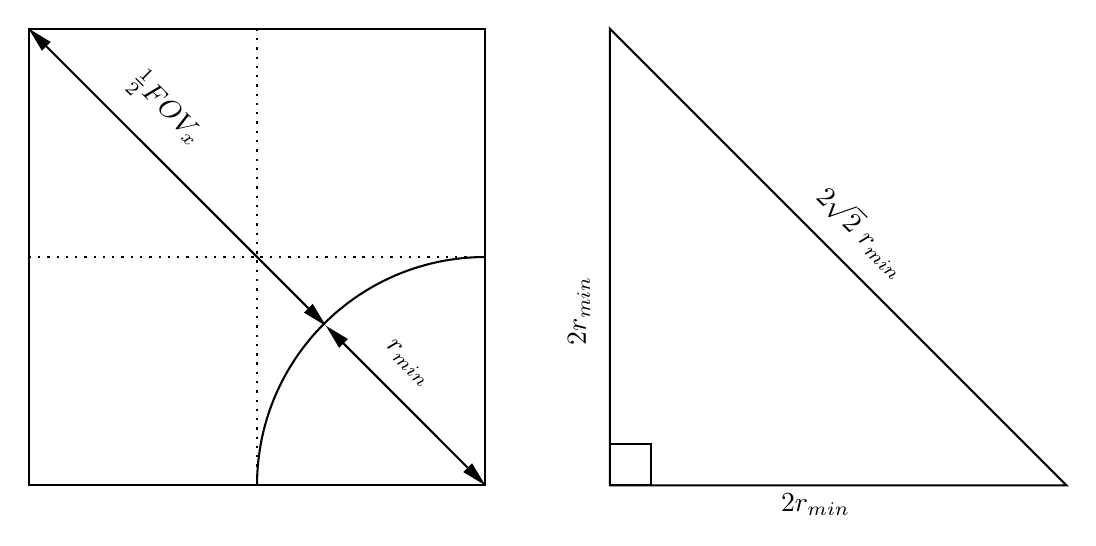
\begin{tikzpicture}[x=0.75pt,y=0.75pt,yscale=-1,xscale=1]
		%uncomment if require: \path (0,464); %set diagram left start at 0, and has height of 464
		
		%Shape: Square [id:dp21273854123077562] 
		\draw  [line width=0.75]  (59,80) -- (279,80) -- (279,300) -- (59,300) -- cycle ;
		%Straight Lines [id:da03805299191386524] 
		\draw [line width=0.75]  [dash pattern={on 0.84pt off 2.51pt}]  (169,80) -- (169,300) ;
		%Straight Lines [id:da4291514540511687] 
		\draw [line width=0.75]  [dash pattern={on 0.84pt off 2.51pt}]  (59,190) -- (279,190) ;
		%Shape: Arc [id:dp32305088211851984] 
		\draw  [draw opacity=0][line width=0.75]  (169,300) .. controls (169,239.25) and (218.25,190) .. (279,190) -- (279,300) -- cycle ; \draw  [line width=0.75]  (169,300) .. controls (169,239.25) and (218.25,190) .. (279,190) ;
		%Straight Lines [id:da34774498940242626] 
		\draw [line width=0.75]    (60.41,81.41) -- (200.78,221.74) ;
		\draw [shift={(202.2,223.15)}, rotate = 224.99] [fill={rgb, 255:red, 0; green, 0; blue, 0 }  ][line width=0.08]  [draw opacity=0] (12,-3) -- (0,0) -- (12,3) -- cycle    ;
		\draw [shift={(59,80)}, rotate = 44.99] [fill={rgb, 255:red, 0; green, 0; blue, 0 }  ][line width=0.08]  [draw opacity=0] (12,-3) -- (0,0) -- (12,3) -- cycle    ;
		%Straight Lines [id:da24453213307250365] 
		\draw [line width=0.75]    (203.61,224.56) -- (277.59,298.59) ;
		\draw [shift={(279,300)}, rotate = 225.02] [fill={rgb, 255:red, 0; green, 0; blue, 0 }  ][line width=0.08]  [draw opacity=0] (12,-3) -- (0,0) -- (12,3) -- cycle    ;
		\draw [shift={(202.2,223.15)}, rotate = 45.02] [fill={rgb, 255:red, 0; green, 0; blue, 0 }  ][line width=0.08]  [draw opacity=0] (12,-3) -- (0,0) -- (12,3) -- cycle    ;
		%Shape: Right Triangle [id:dp960720423813475] 
		\draw  [line width=0.75]  (339,80) -- (559,300) -- (339,300) -- cycle ;
		%Shape: Square [id:dp6932539999111038] 
		\draw  [line width=0.75]  (359,300) -- (339,300) -- (339,280) -- (359,280) -- cycle ;
		
		% Text Node
		\draw (115,95) node [anchor=north west][inner sep=0.75pt]  [rotate=-45]  {$\frac{1}{2}FOV_{x}$};
		% Text Node
		\draw (235,227.1) node [anchor=north west][inner sep=0.75pt]  [rotate=-45]  {$r_{min}$};
		% Text Node
		\draw (420,302.4) node [anchor=north west][inner sep=0.75pt]    {$2r_{min}$};
		% Text Node
		\draw (317.4,234) node [anchor=north west][inner sep=0.75pt]  [rotate=-270]  {$2r_{min}$};
		% Text Node
		\draw (446.39,150.99) node [anchor=north west][inner sep=0.75pt]  [rotate=-45]  {$2\sqrt{2} \ r_{min}$};
		
		
	\end{tikzpicture}
	\caption{Diagram showing the dimensions necessary to calculate FOV on a square discretisation.}
	\label{fig:corner_cutting_02}
\end{figure}

\begin{equation}
	\label{eqn:r_min}
	\begin{aligned}
		r_{min} = \frac{v^2}{g\tan{(\theta_{max}})}
	\end{aligned}
\end{equation}

\begin{equation}
	\label{eqn:fovx from r_min}
	\begin{aligned}
		\frac{FOV_x}{2} &= 2\sqrt{2}r_{min}-r_{min} &\\
		FOV_x &= r_{min}(4\sqrt{2}-2) &
	\end{aligned}
\end{equation}

\begin{equation}
	\label{eqn:AR}
	\begin{aligned}
		A.R. &= \frac{w_{len}}{h_{len}} &\\
	\end{aligned}
\end{equation}

\begin{equation}
	\label{eqn:fovy from fovx}
	\begin{aligned}
		FOV_y &= \frac{FOV_x}{A.R.}
	\end{aligned}
\end{equation}

\noindent Referring back to Equation \ref{eqn:fov_x}, one can calculate the minimum allowable height for this velocity using the following: 

\begin{equation}
	\label{eqn:H_min}
	\begin{aligned}
		H_{min} = \frac{FOV_x \times f}{w_{len}}
	\end{aligned}
\end{equation}

\noindent Section \ref{sec:ER-ED} chooses the maximum allowable \ac{gsd} of 4cm/px for this application. From this, a maximum allowable height can be calculated using Equation \ref{eqn:max_height_calculation}. Now, any height between $H_{min}$ and $H_{max}$ can be selected. The \ac{fov} at that height can then be calculated using Equations \ref{eqn:fov_x} and \ref{eqn:fov_y}. 

Equation \ref{eqn:fovx from r_min} can then be reformulated to calculate the appropriate size of a square discretisation for this \ac{fov}. The radius in the equation is now the maximum allowable radius for this discretisation. This should be equal to or more than the minimum turning radius, which is limited by the velocity.

\begin{equation}
	\label{eqn:}
	\begin{aligned}
		r_{max} &= \frac{FOV_x}{4\sqrt{2}-2} &\\
		l &= 2r_{max}
	\end{aligned}
\end{equation}

Equation \ref{} can also be reformulated to calculate the minimum required bank angle to turn within this square discretisation at the chosen velocity. It is then the decision of the operator what bank angle to use for the turns. It can be anywhere between this $\theta_{min}$ and $\theta_{max}$. The minimum is limited by the square discretisation, which is ultimately limited by the \ac{gsd}. The maximum is the mechanical limit of the \ac{uav} itself.